\documentclass{standalone}

% graphics
\usepackage{tikz}
\usepackage{pgfplots}
\usepackage{siunitx}

\begin{document}

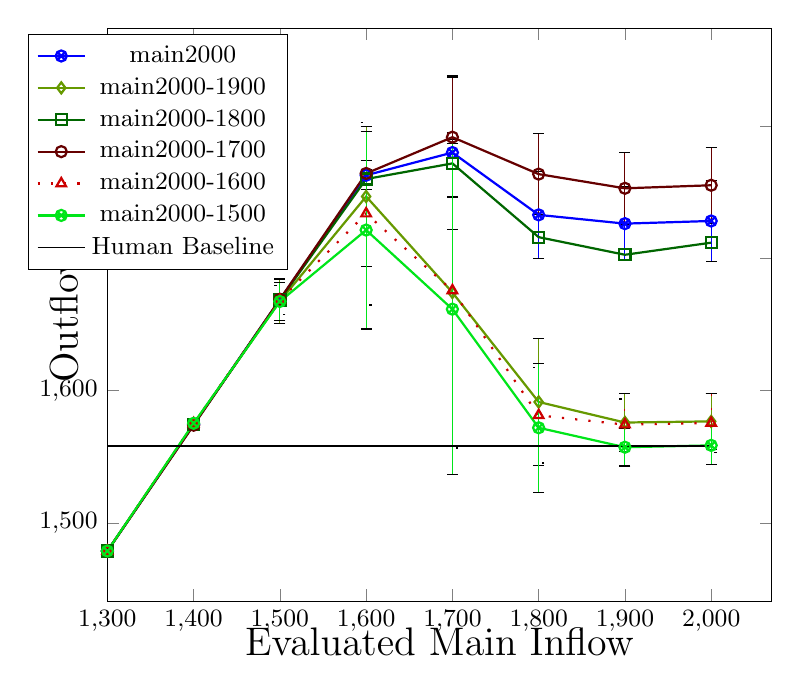
\begin{tikzpicture}[scale=1]
  \pgfplotsset{
      scale only axis,
      every x tick label/.append style={font=\small},
      every y tick label/.append style={font=\small},
	legend style={at={(-0.12,0.99)},anchor=north west}
  }

\begin{axis}[
    legend style={font=\small},
	ylabel={\Large Outflow},
	x label style={at={(axis description cs:0.5,-0.03)},anchor=north},
	y label style={at={(axis description cs:-0.030,0.5)}, anchor=south},
	xlabel={\Large Evaluated Main Inflow},
	xmin=1300
]

%densely dashed, 
%main2000_merge200
\addplot[mark=otimes, thick, mark options={solid, fill=red!60, mark size=2pt},
draw=blue, error bars/.cd, y dir=both, y explicit] table [x=a, y=b, y error=c] {
a	b   	c
1300 1478.74 1.70
1400 1574.35 2.44
1500 1668.85 2.71
1600 1762.88 11.06
1700 1780.06 57.92
1800 1732.93 33.10
1900 1726.31 27.80
2000 1728.32 30.39
};
\label{main2000}



% dashdotdotted,
%main2000-1900_merge200
\addplot[mark=diamond, thick, mark options={solid, fill=blue!40, mark size=2
pt}, draw=green!60!red, error bars/.cd, y dir=both, y explicit] table [x=a, y=b, y error=c] {
a	b   	c
1300 1478.77 1.68
1400 1574.89 2.47
1500 1667.66 16.77
1600 1746.83 52.68
1700 1674.25 115.63
1800 1591.45 48.04
1900 1575.90 21.70
2000 1576.76 21.36
};
\label{main2000-1900}

% error bars/.cd, y dir=both, y explicit,
%main2000-1800_merge200
\addplot[mark=square, thick, mark options={solid, fill=green!60, mark size=2 pt}, draw=black!60!green] table [x=a, y=b] {
a	b   	c
1300 1478.77 1.68
1400 1574.32 2.63
1500 1668.60 6.31
1600 1760.04 21.01
1700 1771.85 70.35
1800 1716.08 39.34
1900 1702.76 30.49
2000 1711.91 28.66
};
\label{main2000-1800}  

%densely dashed, 
%main2000-1700_merge200
\addplot[mark=o, thick, mark options={solid, fill=black!60!red, mark size=2pt}, draw=black!60!red, error bars/.cd, y dir=both, y explicit] table [x=a, y=b, y error=c] {
a	b   	c
1300 1478.70 1.72
1400 1573.88 2.43
1500 1669.10 2.81
1600 1764.25 3.15
1700 1791.68 45.23
1800 1763.75 30.73
1900 1753.02 27.42
2000 1755.32 28.82
};
\label{main2000-1700}

%densely dashed, 
%main2000-1600_merge200
\addplot[mark=triangle, thick, loosely dotted, mark options={solid, fill=red!60, mark size=2pt}, draw=black!20!red, error bars/.cd, y dir=both, y explicit] table [x=a, y=b, y error=c] {
a	b   	c
1300 1478.77 1.68
1400 1575.18 2.30
1500 1668.42 10.83
1600 1733.90 69.11
1700 1675.73 119.12
1800 1581.34 36.08
1900 1574.32 19.36
2000 1575.54 22.51
};
\label{main2000-1600}

%densely dashed, 
%main2000-1500_merge200
\addplot[mark=otimes, thick, mark options={solid, fill=red!60, mark size=2pt},
draw=blue!10!green, error bars/.cd, y dir=both, y explicit] table [x=a, y=b, y error=c] {
a	b   	c
1300 1478.77 1.68
1400 1575.32 2.45
1500 1667.45 14.19
1600 1721.45 74.81
1700 1661.62 125.03
1800 1571.94 48.88
1900 1557.22 14.23
2000 1558.62 14.72
};
\label{main2000-1500}
%
%
%%densely dashed, 
%\addplot[mark=otimes, thick, mark options={solid, fill=blue!60, mark size=2pt},
%draw=blue!10!red, error bars/.cd, y dir=both, y explicit] table [x=a, y=b, y error=c] {
%a	b   	c
%
%};
%\label{linearPPO}
%
\addplot[mark=none, black, samples=200] coordinates {(1300,1558.12)
(2000,1558.12)};
\label{Baseline}


\addlegendimage{/pgfplots/refstyle=main2000}
\addlegendentry{main2000}

\addlegendimage{/pgfplots/refstyle=main2000-1900}
\addlegendentry{main2000-1900}

\addlegendimage{/pgfplots/refstyle=main2000-1800}
\addlegendentry{main2000-1800}

\addlegendimage{/pgfplots/refstyle=main2000-1700}
\addlegendentry{main2000-1700}

\addlegendimage{/pgfplots/refstyle=main2000-1600}
\addlegendentry{main2000-1600}

\addlegendimage{/pgfplots/refstyle=main2000-1500}
\addlegendentry{main2000-1500}

%\addlegendimage{/pgfplots/refstyle=linearPPO}
%\addlegendentry{linearPPOAVP10}

\addlegendimage{/pgfplots/refstyle=Baseline}
\addlegendentry{Human Baseline}




\end{axis}
\end{tikzpicture}

\end{document}

